\part{Applicazioni moderne della crittografia}

\chapter{Identificazione, autenticazione e firma digitale}

\section{Introduzione}
\paragraph{Identificazione} L' \emph{identificazione} prevede che un sistema isolato o in rete debba essere in grado di accertare l'identità di un utente che richiede di accedere ai suoi servizi.

\paragraph{Autenticazione} L' \emph{autenticazione} prevede che il destinatario di un messaggio possa essere in grado di accertare:
\begin{itemize}
    \item l'identità del mittente
    \item l'integrità del crittogramma ricevuto (che non sia stato modificato, che non sia stato sostituito)
\end{itemize}
\paragraph{Attenzione}\[\boxed{\text{Identificazione} \subset \text{Autenticazione}}\]
\paragraph{Firma digitale}
La \emph{firma digitale} ha le seguenti caratteristiche.
\begin{itemize}
    \item \textbf{{Non ripudiabilità}}. Il mittente non può negare di aver inviato il messaggio $m$.
    \item \textbf{{Autenticazione}}. Il destinatario deve essere in grado di autenticare il messaggio.
    \item Il destinatario non deve poter sostenere che $m' \neq m$ è il messaggio inviato dal mittente.
\end{itemize}
Tutto questo deve essere verificabile da terzi (per esempio un giudice)! Non sono modalità indipendenti, ciascuna estende le precedenti! Sono funzionalità utilizzate per contrastare gli attacchi attivi. Ci sono realizzazioni sia su cifrari simmetrici che asimmetrici, noi vedremo queste ultime versioni.

\subsection{Funzioni hash}
Una funzione hash: $f: X \xrightarrow{} Y$ è una funzione tale che:
$$ n = |X| >> m = |Y| $$
La cardinalità del dominio è molto più ampia della cardinalità del codominio. Essendo non iniettiva il codominio potrà essere partizionato in insiemi di elementi del dominio che condividono lo stesso valore hash (con la stessa \emph{collisione}).
$$ \exists\, X_1, X_2, \dots, X_m \subseteq X$$
Gli insiemi sono disgiunti, tali che: 
$$ X = X_1 \cup X_2 \cup \dots \cup  X_m $$
$$ \forall i, x : x \in X_i : f(x) = y $$
\begin{itemize}
	\item Si vuole che le dimensioni dei vari insiemi $X_i$ siano più omogenee possibile: quindi due elementi estratti a caso da $X$ hanno probabilità circa $\frac{1}{m}$ di avere la stessa immagine $y$.
	\item Si vuole che immagini \emph{simili} tra loro appartengano a sottoinsiemi diversi (quindi immagini hash diverse).
	\item Bisogna gestire le collisioni.
\end{itemize}
Non ci bastano queste proprietà in crittografia. 
\subsubsection{Funzioni hash \emph{one-way}}
Per le applicazioni crittografiche si devono avere le seguenti proprietà ($f: X \xrightarrow{} Y$):
\begin{itemize}
    \item $\forall x \in X$ è computazionalmente facile calcolare $$y = f(x)$$
    \item \textbf{Proprietà one-way}. 
    
    Per la maggior parte degli $y \in Y$ è computazionalmente difficile determinare $$x \in X: f(x) = y$$
    \item \textbf{Proprietà {claw-free}}. 
    
    E' computazionalmente difficile determinare $<x_1, x_2>$ in $X$ tale che: $$f(x_1)=f(x_2)$$
    cioè deve essere difficile individuare due elementi che hanno la stessa \emph{collisione}.
\end{itemize}

\subsubsection{MD5 (Message Digest, v5)}
\begin{itemize}
	\item Si tratta di una famiglia di algoritmi. 	Sono stati pubblicati MD2, MD4, MD5. Nei primi due furono trovate falle e Rivest propose MD5 nel 1992.
	
	\item Riceve in input un sequenza $S$ di 512 bit e produce un'immagine di 128 bit.
	
	Si \emph{digerisce} la sequenza riducendone la lunghezza ad $\frac{1}{4}$.
	
	\item Non resiste alle collisioni e nel 2004 è uscito di scena con debolezze varie. Si considera severamente compromesso (anche dallo stesso Rivest).
	
	Si usa ancora in altri contesti non crittografici.
\end{itemize}

\subsubsection{RIPEMD-160}
E' la versione matura del \emph{Message Digest} (MD*). Nata nel 1995 produce immagini di 160 bit e non presenta i difetti di MD5.

\subsubsection{SHA (Secure Hash Algorithm)}
\begin{itemize}
	\item Progettata dal NIST ed NSA nel 1993 (enti statunitensi).
	\item Opera su sequenze lunghe fino a $2^{64}$ bit e produce immagini di 160 bit.
	\item \textbf{E' crittograficamente sicura}.
	\begin{itemize}
		\item La prima versione: SHA-0 conteneva debolezze e fu quindi rivista portando allo SHA-1.
		
		\item Sono poi stati creati SHA-2: altri 4 algoritmi caratterizzati da digest più lunghi.
		
		\item Nel 2007 a causa dei problemi di MD5 e SHA-0 il NIST ha richiesto nuovi standard e nel 2012 è stato selezionato un algoritmo che è diventano SHA-3, pubblicato ufficialmente nel 2015.
	\end{itemize}
\end{itemize}

\paragraph{SHA-1 a titolo di esempio}
\begin{itemize}
	\item 
	Opera su sequenze fino a $2^{64}-1$ bit e produce immagini di 160 bit.
	E' largamente usata nei protocolli crittografici anche se non è più certificata come standard.
	
	\item Opera su blocchi di 160 bit contenuti in un buffer di 5 registri da 32 bit ciascuno in cui sono caricati inizialmente dei valori pubblici.
	Il messaggio $m$ viene poi concatenato con una sequenza di padding che ne rende la lunghezza multipla di 512 bit.
	
	\item Il contenuto dei registri varia nel corso dei cicli successivi in cui questi valori si combinano tra loro e con blocchi di 21 bit provenientei da $m$.
	Alla fine i registri contengono SHA-1($m$).
\end{itemize}
\begin{center}
	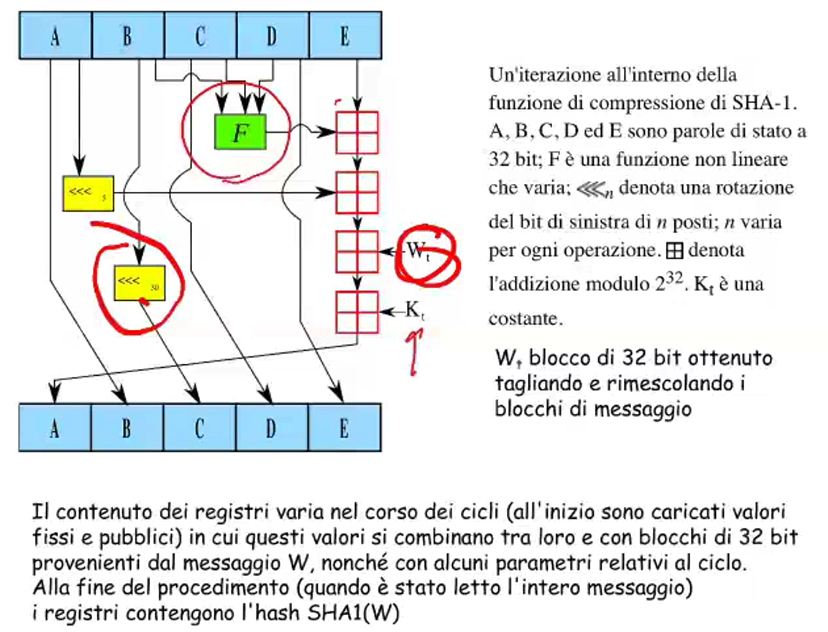
\includegraphics[scale=.65]{images/33.PNG}
\end{center}

\section{Protocollo di identificazione su canali sicuri}
Supponiamo di trovarci in un canale sicuro, cioè un canale protetto in lettura e scrittura, inaccessibile ad esterni indesiderati. Supponiamo di avere un utente che vuole accedere alle risorse su un calcolatore: per identificarsi utilizza \emph{username} e \emph{password}.
\paragraph{hash} Sono possibili attacchi da utenti interni, che potrebbero accedere al database e leggere le password. Per evitare problemi di questo tipo non si memorizzano mai le password in chiaro, ma un valore \emph{hash}.
\paragraph{Esempio UNIX} Quando un utente $U$ fornisce per la prima volta una password $P$ il sistema UNIX associa ad $U$ due sequenze binarie (\textbf{LE MEMORIZZA NEL FILE DELLE PASSWORD} al posto della password vera e propria, ricordare quanto visto a Sistemi Operativi):
\begin{itemize}
    \item $S$, un seme prodotto mediante generatore pseudocasuale;
    \item $Q = h(PS)$, hash della concatenazione di $P$ ed $S$.
\end{itemize}
Ad ogni successiva connessione il sistema:
\begin{itemize}
	\item prende l'hash $S$ dal file delle password e la password $P'$ \textbf{\underline{trasmessa}} dall'utente;
	\item li concatena ed applica la funzione hash.
\end{itemize} 
Se il risultato della funzione hash è uguale a $Q$ (posto sempre nel file delle password) allora avviene il riconoscimento.
\pagebreak
\begin{center}
	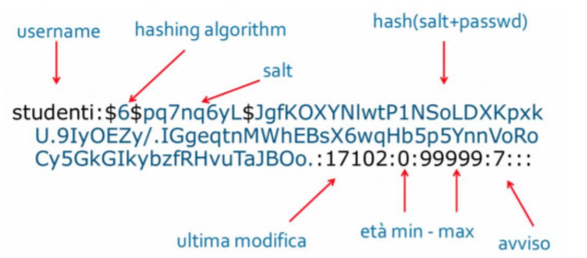
\includegraphics[scale=.85]{images/34.PNG}
\end{center}
\paragraph{Utilità} In questa maniera un accesso al file delle password non rivela informazioni importanti.

\section{Protocollo di identificazione su canali insicuri}
Se il canale è insicuro l'utente che vuole accedere la servizio non può trasmettere la password sul canale stesso: potrebbe essere intercettata durante la sua trasmissione in chiaro! Vediamo quindi un sistema di \emph{identificazione} basato su chiave pubblica e privata.

\paragraph{Sistema proposto} Per esempio siano $<e,n>$, $<d,n>$ le chiavi pubblica e privata di un utente $U$ (stessa struttura vista nell'RSA), che richiede l'accesso ai servizi offerti dal sistema $S$.
\begin{itemize}
    \item Il sistema $S$ genera un numero casuale $r < n$ e lo invia in chiaro a $U$
    \item L'utente $U$ calcola la \emph{firma di $U$ su $r$} \underline{utilizzando la chiave privata $d$}
    $$ f = r^d \text{ mod } n $$
    invia questo valore al sistema $S$
    \item Il sistema $S$ verifica la correttezza del valore ricevuto dall'utente $U$ calcolando:
    $$ f^e \text{ mod }  n =r$$
    Verifica l'uguaglianza. In caso di corrispondenza l'identificazione ha successo
\end{itemize}
\paragraph{Problema: sistemi non fidati} Se il sistema $S$ non è \emph{trusted} questo potrebbe inviare un $r$ particolare, anziché randomico, per cercare di carpire informazioni sulla chiave privata! La questione sarà affrontata col protocollo \emph{Zero Knowledge}.

\paragraph{Inversione rispetto all'RSA} Le operazioni di criptazione e decifrazione sono invertite (prima viene usata la chiave privata e poi la chiave pubblica) rispetto all'RSA. Ciò è possibile grazie alla seguente proprietà commutativa.
$$ (x^e \text{ mod } n)^d \text{ mod } n = (x^d \text{ mod } n)^e \text{ mod } n = x $$
Inoltre $f$ può essere generata solo dall'utente $U$ che possiede la chiave privata $<d,n>$. 

\section{Autenticazione su canale insicuro}
\subsection{Protocollo}
Per eseguire l'autenticazione invece si usa il MAC: \emph{message authentication code}.
\begin{itemize}
    \item Mittente e destinatario concordano una chiave segreta $k$
    \item Il mittente allega al messaggio un MAC:
    $$ A(m,k) $$
    allo scopo di garantire la provenienza e l'integrità del messaggio. Lo spedisce in coppia col messaggio in chiaro oppure col crittogramma
    \begin{align*}
    	<m, A(m,k)> && <C(m,k'),A(m,k)>
    \end{align*}
    \item Il destinatario entra in possesso di $m$, conosce il MAC $A(m,k)$ e ha già concordato la chiave $k$ col suo interlocutore (non è mai passata dal canale insicuro, quindi il crittoanalista non può conoscerla). Ricalcola $A(m,k)$ usando il messaggio $m$ ricevuto e ne confronta il valore col MAC inviato dal mittente. 
\end{itemize}
Se i MAC corrispondono allora l'autenticazione ha successo.

\subsection{\emph{Message Authentication Code} (MAC)}
Il \emph{Message Authentication Code} deve essere una immagine breve del messaggio, generabile solo se si consoce il valore $k$ (lo conoscono solo i due interlocutori). Ci sono varie implementazioni basate su cifrari asimmetrici, simmetrici e funzioni hash one-way. In particolare la versione one-way prevede:
$$ A(m,k) = h(mk) $$
con $h$ una \emph{funzione hash one-way}.

\paragraph{Sicurezza} E' sicuro in quanto $k$ viaggia nel MAC ed anche se venisse scoperto non è invertibile in maniera semplice.
Non può nemmeno sostituire tutto in quanto dovrebbe corredare il messaggio di un nuovo MAC che però non può calcolare essendo all' oscuro del valore di $k$.

\paragraph{Alternativa} Alternativa alle funzioni hash one-way, in un cifrario a blocchi in modalità CBC, è l'uso dell'ultimo blocco come MAC. La cosa è lecitissima in quanto la sequenza ottenuta rappresenta l'intero messaggio.

\section{Protocolli per la firma digitale}
\subsection{Caratteristiche della firma manuale e di quella digitale}
Riflettiamo sulle caratteristiche della firma manuale, da "traslare" nella firma digitale:
\begin{itemize}
    \item è autentica e non falsabile, prova che chi la ha prodotta è chi ha sottoscritto il documento;
    \item non è riutilizzabile, è legata al documento su cui è stata apposta;
    \item il documento non è alterabile, chi ha prodotto la firma è sicuro che questa si riferirà solo al documento sottoscritto nella sua forma originale;
    \item non può essere ripudiata da chi l'ha apposta costituendo prova legale di un accordo o dichiarazione.
\end{itemize}
Nella firma digitale si deve tenere conto delle cose già dette (autenticazione in primis) e di un altro dettaglio: essa non è la digitalizzazione della firma manuale, ma un qualcosa a se stante (essa non può essere la digitalizzazione di un documento originale firmato manualmente). Farla dipendere dalla firma manuale significa ridurne il potenziale. Ci sono protocolli che si basano sia su cifrari simmetrici che asimmetrici.

\subsection{Protocollo 1: messaggio in chiaro e firmato (DH)}
L'utente $U$ dispone di una $K_{upriv}$ e $K_{upub}$. $C$ e $D$ sono funzioni di cifratura e decifratura di un cifrario asimmetrico.
La firma funziona:
\begin{itemize}
    \item \textbf{Generazione della firma}.
    
    $U$ genera la firma decifrando il messaggio in chiaro
    $$f = D(m, k_{upriv})$$
    e spedisce all'utente $<U,m,f>$, dove $U$ è l'identificativo dell'utente
    \item \textbf{Verifica della firma}.
    
    L'utente riceve $<U,m,f>$, cifra il valore $f$ 
    $$C(f, K_{upub}) = m$$
    e verifica che il risultato sia proprio $m$
\end{itemize}
L'indicazione del mittente $U$ consente a $V$ di selezionare la $K_{upub}$ da utilizzare. Per far funzionare questo meccanismo è importante che $C$ e $D$ siano commutative, cioè
$$C(D(m))=D(C(m))=m$$

\paragraph{Requisiti della firma digiale} Questo protocollo soddisfa i requisiti della firma digitale. Si pensi a quali elementi influenzano la generazione della firma digitale: il messaggio $m$ e la chiave privata (quindi l'utente $U$, la chiave privata è nota solo a lui). 
\begin{itemize}
    \item E' autentica e non falsabile: $K_{upriv}$  è nota solo al mittente
    \item Il documento non può essere alterato in quanto $m$ e $f$ sarebbero inconsistenti
    \item $U$ non può ripudiare la firma perché \textbf{può averla prodotta solo lui}
    \item La firma non è riutilizzabile in quanto $f$ è immagine di $m$.
\end{itemize}

\subsection{Protocollo 2: messaggio cifrato e firmato}
Per trasmettere un crittogramma è necessario alterare il protocollo precedentemente introdotto: se cifriamo il crittogramma nella verifica della firma si restituisce il messaggio in chiaro, e la verifica della firma richiede la sola chiave pubblica. 
\paragraph{Firma e cifratura} Si distingua chiave di $U$ da chiave di $V$
\begin{itemize}
    \item $U$ genera la firma sempre a partire dal messaggio $m$ e dalla chiave privata sua:
    $$ f = D(m, K_{upriv}) $$
    \item Si calcola il crittogramma della firma appena generata con la chiave del destinatario.
    $$ c = C(f, K_{vpub}) $$
    \item Invia $<U, c>$, dove $U$ è l'identificativo dell'utente
\end{itemize}
\paragraph{Decifrazione e verifica} 
\begin{itemize}
	\item L'utente $V$ riceve la coppia $<U, c>$ e la decifra con la chiave privata sua:
	$$ D(c, K_{vpriv}) = f $$
	\item Verificando la firma (chiave pubblica del mittente) si ottiene anche il messaggio:
	$$ C(f, K_{upub}) = C(D(m, K_{upriv}), K_{upub}) = m $$
\end{itemize}
\subsubsection{Schema applicato all'RSA}
Per quanto riguarda le chiavi immaginiamoci il solito schema, sia per $U$ che per $V$. L'utente U, che vuole scrivere a $V$, fa i primi passi:
\begin{itemize}
    \item firma il messaggio $f = m^{d_u} \mod n_u$ (usa la chiave privata di $U$, cioè $<d_u,n_u>$);
    \item cifra il messaggio $c = f^{e_v} \mod n_v$ (usa la chiave pubblica di $V$, cioè $<e_v,n_v>$);
    \item spedisce la coppia ottenuta $<U, c>$;
\end{itemize}
L'utente V:
\begin{itemize}
    \item riceve e decifra $f = c^{d_v} \mod n_v$ (usa la chiave privata di $V$, cioè $<d_v,n_v>$);
    \item decifra $f$ con $k_{upub}$, $f^{e_u} \mod n_u = m$ (usa la chiave pubblica di $U$, cioè $<e_u,n_u>$).
\end{itemize}
Se $m$ è significativo concludo che è autentico.

\paragraph{Osservazioni} 
\begin{itemize}
	\item Per la correttezza del procedimento è necessario che $n_u \leq n_v$ affinché sia vero che $f < n_v$ e quindi $f$ possa essere cifrato correttamente.
	In questo modo tuttavia $V$ non può rispondere in quanto dovrebbero avere $n_u = n_v$ ma è poco sicuro e probabile.
	\item Possiamo ovviare quindi dando ad ogni utente due chiavi distinte: \begin{itemize}
		\item una per la firma $< H$ 
		\item una per la cifratura $> H$
	\end{itemize}  con $H$ pubblico e molto grande.
	NB: si può attaccare se ci si procura la firma di un utente su un messaggio apparentemente privo di senso
\end{itemize}


\subsubsection{Attacco con giochi algebrici}
Supponiamo che un utente $U$ abbia l'abitudine di inviare una risposta automatica (ack) al mittente ogni volta che riceve un messaggio $m$, e che questo messaggio sia il crittogramma della firma di $U$ su $m$.
\paragraph{Crittoanalista} Un crittoanalista attivo $X$ può decifrare i messaggi inviati a U:
\begin{itemize}
    \item $X$ intercetta $c$ firmato e crittografato inviato da $V$ a $U$, lo rimuove dal canale e lo rispedisce a $U$ con identificativo $X$. (cancella $<V,c>$ ed invia $<X,c>$)
    \item $U$ spedisce un ack ad $X$ in risposta
    \item $X$ usa l' ack per risalire al messaggio $m$ applicando le funzioni del cifrario con le chiavi pubbliche di $V$ e di $U$.
\end{itemize}
In particolare succede:
\begin{itemize}
    \item $V$ invia $c$ a $U$:
        $$
            \begin{cases}
                c = C(f, K_{upub}) \\
                f = D(m, K_{vpriv})
            \end{cases}
            \implies <V,c>
        $$
    \item $X$ intercetta la coppia, la rimuove dal canale prima che possa essere consegnata al destinatario, invia all'utente $U$ la coppia $<X,c>$
    \item $U$ riceve la coppia $<X,c>$ decifra $c$:
    $$ f = D(c, K_{upriv}) $$
    e verifica la firma con la chiave pubblica di X ottenendo:
    $$ m' = C(f, K_{xpub}) $$
    Il messaggio $m'$ ottenuto è privo di senso ($m' \neq m$) perchè la generazione della chiave non è avvenuta con la chiave di $X$, ma con quella di $V$. 
    \item Nonostante l'inconsistenza del messaggio l'utente $U$ l'ack $c'$ ad $X$:
    $$ f' = D(m', K_{upriv}) \Longrightarrow c' = C(f', K_{xpub}) $$
    \item \textbf{Giochini algebrici}.
    
    Il crittoanalista $X$ usa $c'$ ricevuto da $U$ per risalire ad $m$: decifra (con la chiave privata del crittoanalista) $$c': D(c', K_{xpriv}) = f'$$ e verifica (con la chiave pubblica del destinatario) $$f': C(f', K_{upub}) = m'$$Da $m'$ ricava (chiave privata del crittoanalista) $$f: D(m', K_{xpriv})=f$$verifica (chiave pubblica del vero mittente)$$f: C(f, K_{vpub}) = m$$
\end{itemize}
Attraverso questi giochini l'utente ha ottenuto $f$, e a quel punto tutto è in discesa: basta conoscere la chiave pubblica di $V$! Per evitare l'attacco si deve evitare l'ack automatico.

\subsection{Protocollo resistente agli attacchi}
Si evita di firmare il messaggio!
Si crea un hash del messaggio (SHA) con una funzione hash one-way e vi si appone la firma sopra.
La firma non è quindi più soggetta ai giochi algebrici appena visti.
\paragraph{Generazione della firma e cifratura}
\begin{itemize}
    \item il mittente $U$ calcola $h(m)$ e genera:
    $ f = D(h(m), K_{upriv})$
    \item calcola separatamente:
    $c = C(m, K_{vpub}) $
    \item spedisce a $V$ la tripla: $<U, c, f>$
\end{itemize}
\paragraph{Decifrazione e verifica}
\begin{itemize}
    \item $V$ riceve e verifica $<U, c, f>$
    \item decifra il crittogramma $c: m = D(c, K_{upriv})$
    \item calcola $h(m)$ (conosce la funzione \emph{hash} come il suo interlocutore) e $C(f, K_{upub})$ (conosce la chiave pubblica dell'interlocutore) e ne controlla l'uguaglianza, se sono uguali il messaggio è autentico
\end{itemize}
La firma si calcola più velocemente.

\subsection{Attacchi man-in-the-middle}
Le chiavi di cifratura sono pubbliche e non richiedono un incontro diretto per il loro scambio.
Un crittoanalista attivo può quindi intromettersi \textbf{\underline{nella fase iniziale}} comportandosi come $V$ agli occhi di $U$ e come $U$ agli occhi di $V$.
\begin{itemize}
    \item $U$ richiede a $V$ la sua chiave pubblica
    \item $X$ intercetta la risposta con $K_{vpub}$ e la sostituisce con la sua chiave pubblica $K_{xpub}$
    \item $X$ si pone in attesa dei crittogrammi spediti da $U$ a $V$ cifrati mediante $K_{xpub}$
    \item $X$ rimuove dal canale ciascuno dei crittogrammi, li decripta e li cifra con $K_{vpub}$ trafugata all'inizio, rispedendola a $V$
    \item $U$ e $V$ non si accorgono di nulla se il tutto è fatto velocemente
\end{itemize}
La cosa si risolve introducendo la \emph{Certification Authority}.

\section{Certification Authority - CA}
Sono infrastrutture/enti che garantiscono la validità delle chiavi pubbliche e ne regolano l'uso gestendo la distribuzione delle chiavi a chi vuole comunicare.
La CA autentica l'associazione emettendo un certificato digitale$$<\text{utente}, \text{chiave pubblica}>$$ 
Il certificato consiste della chiave pubblica e di una lista di informazioni relative al suo proprietario opportunamente firmate dalla CA. Mantiene quindi un archivio accessibile a tutti ma protetto da scritture non autorizzate. La chiave della CA è nota agli utenti che la mantengono protetta e la utilizzano per verificare la firma della stessa CA.

\subsection{Contenuto del certificato digitale}
Si compone principalmente di:
\begin{itemize}
    \item indicazione del formato (numero di versione)
    \item nome della CA che lo ha rilasciato
    \item numero seriale che lo individua univocamente nella CA emittente
    \pagebreak 
    \item specifica dell'algoritmo usato dalla CA per creare la firma digitale
    \item periodo di validità
    \item nome ed altre informazioni dell'utente a cui si riferisce il certificato
    \item nome dell'algoritmo, parametri e chiave pubblica usati dall'utente per cifr. e firm.
    \item firma della CA su tutto quanto
\end{itemize}
Quindi:
\begin{itemize}
	\item 
	Se $U$ vuole comunicare con $V$ può richiedere $K_{vpub}$ alla CA oppure direttamente a $V$ e poi lo convalida tramite la CA.
	
	\item Dato che $U$ conosce $K_{CA-pub}$ può controllarne l'autenticità e la validità.
	
	\item Ci si può mettere nel mezzo solo falsificando la certificazione ma si assume che la CA sia fidata.
	
	\item Esistono varie CA organizzate ad albero, la verifica quindi è più complicata in quanto si cerca il primo antenato comune tra le CA di $U$ e di $V$. Ogni utente poi mantiene in cache una copia dei certificati richiesti ed una copia di $K_{CA-pub}$ per non doverla richiedere.
\end{itemize}

\section{Protocollo finale con certificazione digitale}
\paragraph{Mittente} Il mittente $U$:
\begin{enumerate}
    \item si procura $cert$ di V (dove è presente la chiave con cui calcoliamo $c$)

    \item calcola $h(m)$ (con la sua chiave privata) e firma:
    $$ f = D(h(m),K_{upriv}) $$

    \item calcola $c$ (usando la chiave pubblica del destinatario, ottenuta dal certif. digitale):
    $$ c = C(m, K_{vpub}) $$

    \item spedisce la terna $<cert_U$, c, f$>$ ($cert_U$ contiene $K_{upub}$, quindi non è necessario trasmetterla separatamente)
\end{enumerate}
\paragraph{Destinatario} Il destinatario $V$:
\begin{itemize}
    \item riceve $<cert_U$, c, f$>$ e verifica l'autenticità di $cert_U$ (e di $K_{upub}$) tramite la CA.

    \item decifra il crittogramma:
    $$ m=D(c, K_{vpriv}) $$

    \item verifica l'autenticità della firma:
    $$ C(f, K_{upub}) = h(m) $$
\end{itemize}
\paragraph{Attenzione} La catena ha un punto debole: i certificati non più validi; è quindi cruciale controllare periodicamente con la CA i certificati scaduti.